\documentclass[10pt]{article}
\usepackage[left=1in,right=1in,top=0.9in,bottom=1in]{geometry}
\usepackage{algorithm}
\usepackage{algpseudocode}
\usepackage{amsmath}
\usepackage{amssymb}
\usepackage{graphicx}
\usepackage{float}
\usepackage{mathptmx}
\usepackage{hyperref}
\usepackage[linesnumbered,ruled,vlined]{algorithm2e}
\usepackage{caption}
\usepackage[most]{tcolorbox}
\usepackage{listings}
\usepackage{inconsolata}
\usepackage{xcolor}


\definecolor{codebg}{RGB}{245,245,245}
\definecolor{codeframe}{RGB}{200,200,200}
\lstdefinelanguage{CustomC++}[]{C++}{
    morekeywords={constexpr, nullptr, noexcept, auto, class, public, private, virtual, override},
}

\lstset{
    language=CustomC++,
    backgroundcolor=\color{codebg},
    basicstyle=\ttfamily\small,     % Consolas-like font
    keywordstyle=\color{blue}\bfseries,
    stringstyle=\color{orange},
    commentstyle=\color{gray}\itshape,
    numberstyle=\tiny\color{gray},
    numbers=left,
    stepnumber=1,
    numbersep=10pt,
    frame=single,
    rulecolor=\color{codeframe},
    showstringspaces=false,
    tabsize=4,
    breaklines=true,
    captionpos=b
}

\title{Comparison of BTO, MVTO, MVTO-gc, k-MVTO}
\author{Name: Tushita Sharva\\Roll Number: CS21BTECH11022}
\date{\today}

\begin{document}

\maketitle

\section{Problem Statement}
This project implements and compares the scheduling algorithms: BTO, MVTO, k-MVTO, MVTO-gc. The performance is measured in terms of:
\begin{itemize}
    \item The average number of times a transaction is aborted before committing (abort count).
    \item The average time taken for a transaction to commit (commit delay).
\end{itemize}

\paragraph{Parameters}
\begin{itemize}
    \item $n$: Number of threads.
    \item $m$: Number of shared data items.
    \item $totalTrans$: Total number of committed transactions required.
    \item $constVal$: Parameter for simulating increment operations on data items.
    \item \textbf{$\lambda$}: Parameter for simulating complex operations in transactions.
    \item \textbf{$numIters$}: Number of read and write actions per transaction.
\end{itemize}

\section{Program Design}
The project consists of several classes implemented in C++.

\subsection{Classes \& Their Methods}
\subsubsection{Logger Class}
Handles logging for output and debugging. Provides time-stamped log entries for transaction execution and validation.

\subsubsection{Transaction Class}
Maintains attributes of a transaction. Key members:
\begin{itemize}
    \item \textbf{id}: Unique transaction identifier.
    \item \textbf{status}: Transaction state (active, committed, aborted).
    \item \textbf{localSharedMemory}: Stores local modifications before committing.
\end{itemize}

\subsubsection{DataItem Class}
Encapsulates shared data items and tracks transactions accessing them. I implemented separate classes, one for BTO protocol, called \texttt{PrimitiveDataItem.h} and one for variants of MVTO protocol, called \texttt{DataItem.h}. \texttt{DataItem.h} uses another class \texttt{VersionedDataItem.h}, which has the details of specific version.
Classes are as follows:
\begin{lstlisting}
class DataItem { // For BTO
public:
    int value;
    int maxRead;
    int maxWrite;
    std::mutex datalock;

    DataItem() {
        value = 0;
        maxRead = INT_MIN;
        maxWrite = INT_MIN;
    }
};
\end{lstlisting}

\begin{lstlisting}
class VersionedDataItem {
public:
    int version;
    int valueInThisVersion;
    std::set<int> readList;

    int getLargestInReadList();
};
\end{lstlisting}

\begin{lstlisting}
class DataItem { // M
public:
    std::map<int, VersionedDataItem> versions;  // key = version
    std::mutex datalock;

    DataItem() { // Initialize with a 0th version }
    int getGreatestVersionLessThanMyId(int id);
};
\end{lstlisting}

\section{Validation logics for the protocols}
\paragraph{BTO:}
\begin{itemize}
    \item Whenever a transaction reads a data item, scheduler checks with the maxWrite of the data item and if it's time stamp is less, it is aborted.
    \item Whenever a tranction writes a data item, scheduler checks with both maxRead and maxWrite of the data item, and if it's time stamp is less and it hasn't written to it before, it is aborted.
    \item \textbf{Here, when a second read/write comes, I am not checking if it is validity, but directly accessing the local memory. This is because since we are going in an optimistic way and we are writing at the end of transaction, why don't we modify the local value and write the same at the end? It seems logical even because page model allows only one read and one write per data item per transaction.}
\end{itemize}


\paragraph{MVTO:}
\begin{itemize}
    \item When we read, we see if it is local shared memory, else we read from the smallest version less than ourselves. There won't be any aborts caused by a \texttt{read} in this algorithm.
    \item When we write, we see if the write is valid, and if not, we abort. If it is valid, we write to the local memory.
    \item When the transaction is trying to commit, we check if the transaction is ongoing. If it is not, we abort. If it is valid, we write to the shared memory, by adding a new version to each data item we accessed.
\end{itemize}

\paragraph{k-MVTO:}
\begin{itemize}
    \item When we read, we see if it is local shared memory, else we read from the smallest version less than ourselves. We abort the transaction if we cannot find a version less than ourselves.
    \item When we write, we see if the write is valid, and if not, we abort. If it is valid, we write to the local memory.
    \item When the transaction is trying to commit, we check if the transaction is ongoing. If it is not, we abort. If it is valid, we write to the shared memory, by adding a new version to each data item we accessed. If the number of versions exceeds $k$, we remove the oldest version.
\end{itemize}

\paragraph{MVTO-gc:}
\begin{itemize}
    \item When we read, we see if it is local shared memory, else we read from the smallest version less than ourselves.
    \item When we write, we see if the write is valid, and if not, we abort. If it is valid, we write to the local memory.
    \item When the transaction is trying to commit, we check if the transaction is ongoing. If it is not, we abort. If it is valid, we write to the shared memory, by adding a new version to each data item we accessed.
    \item Whenever a transaction commits, it checks the smallest live transaction from the live set. We also keep a variable smallest live transaction, initialised with 0. Whenver a transaction commits, it checks if the smallest live transaction in the live set is same as the one that was seen by a previously committed transaction. If it changed, \textbf{only then} the transaction performs garbage collection. And whenever a transaction observes the smallest live transaction changed, it updates the variable.
    \item If we donot keep an extra variable, we will access every data item and find that there is no version less than the smallest live transaction and return without performing any. Even though this is O(1) time, this time will be multiplied with number of shared variables, hence saves time.
\end{itemize}

\pagebreak
\section{Experimental Results}

\subsection{Experiment 1: Varying number of transactions || 16 threads}
\begin{figure}[h]
    \centering
    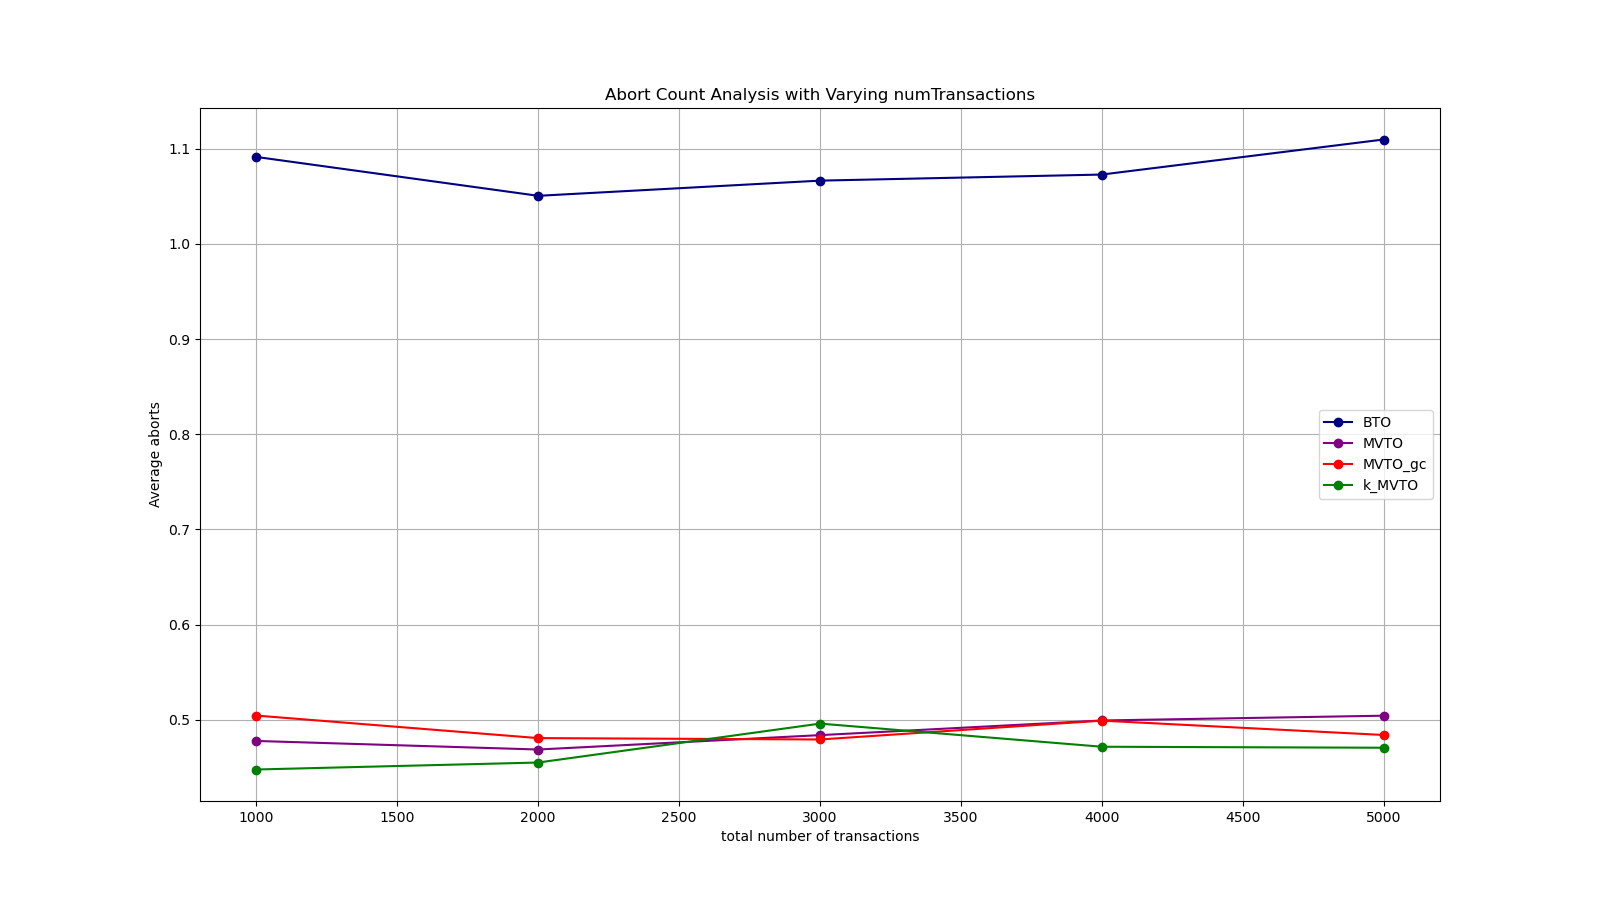
\includegraphics[width=0.9\linewidth]{img/E1_abortCount.png}
\end{figure}

\begin{figure}[h]
    \centering
    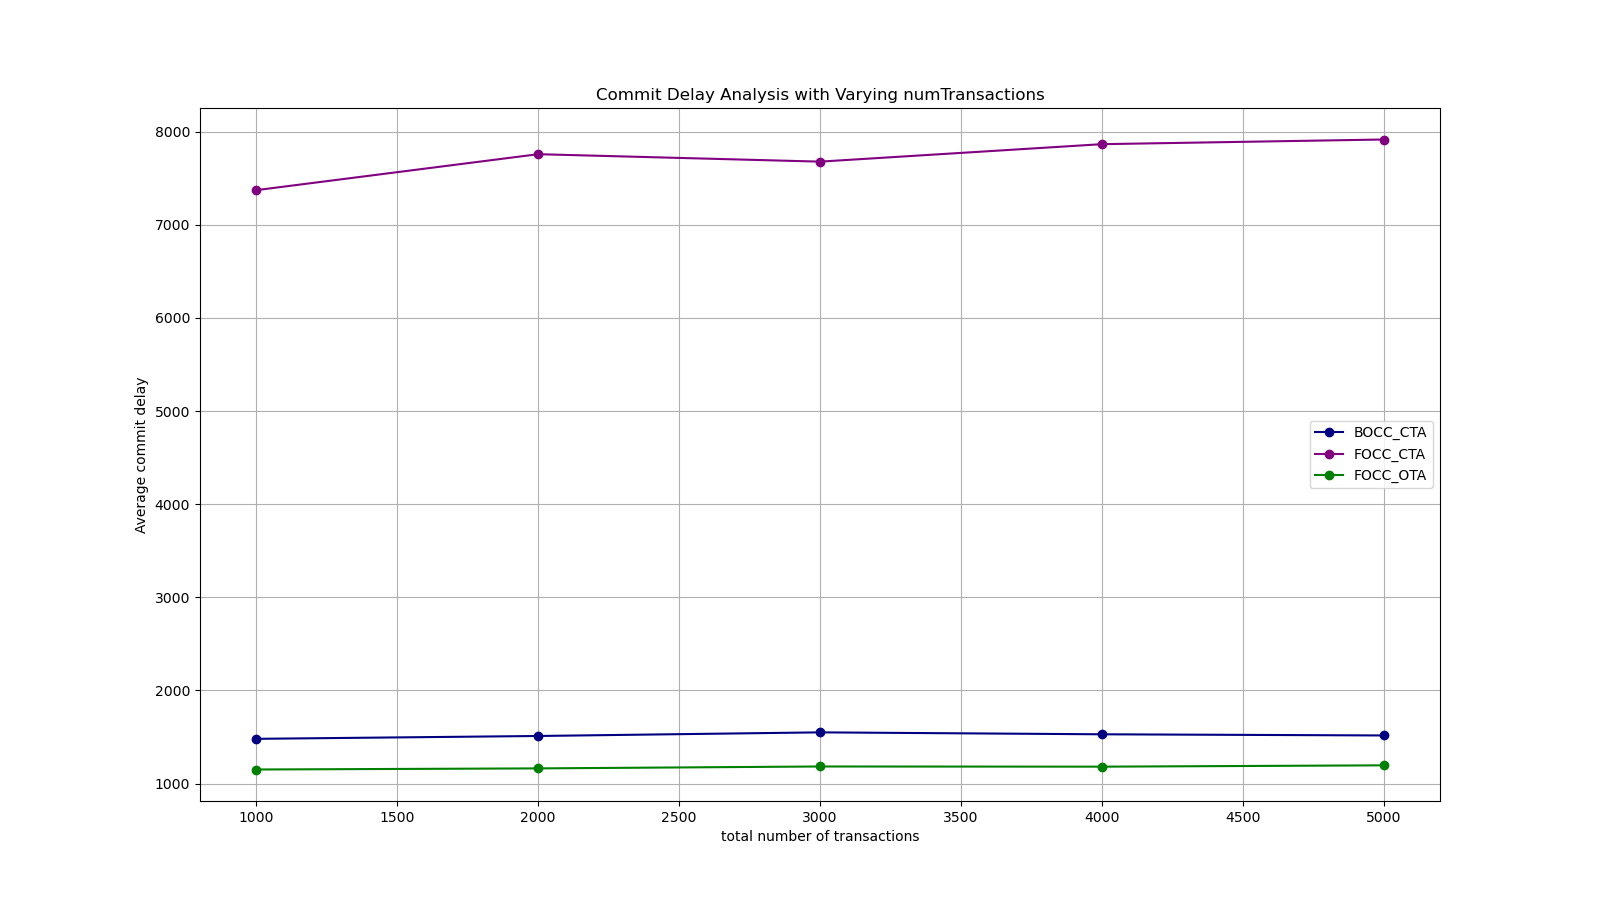
\includegraphics[width=0.9\linewidth]{img/E1_commitDelay.png}
\end{figure}
\paragraph{Explanation} We can see that BTO performs the worst, because of more number of aborts the algoroithm causes. The performance of all three variants of MVTO are comparable, with k-MVTO outperforming others most of the times! This is a bit surprising because k-mvto is the one which has fixed number of versions and also causes aborts even in read-only transactions. However, this isn't observed here. This can be attributed to the randomness caused by readRatio.


\subsection{Experiment 2: Varying number of shared variables}
\begin{figure}[h]
    \centering
    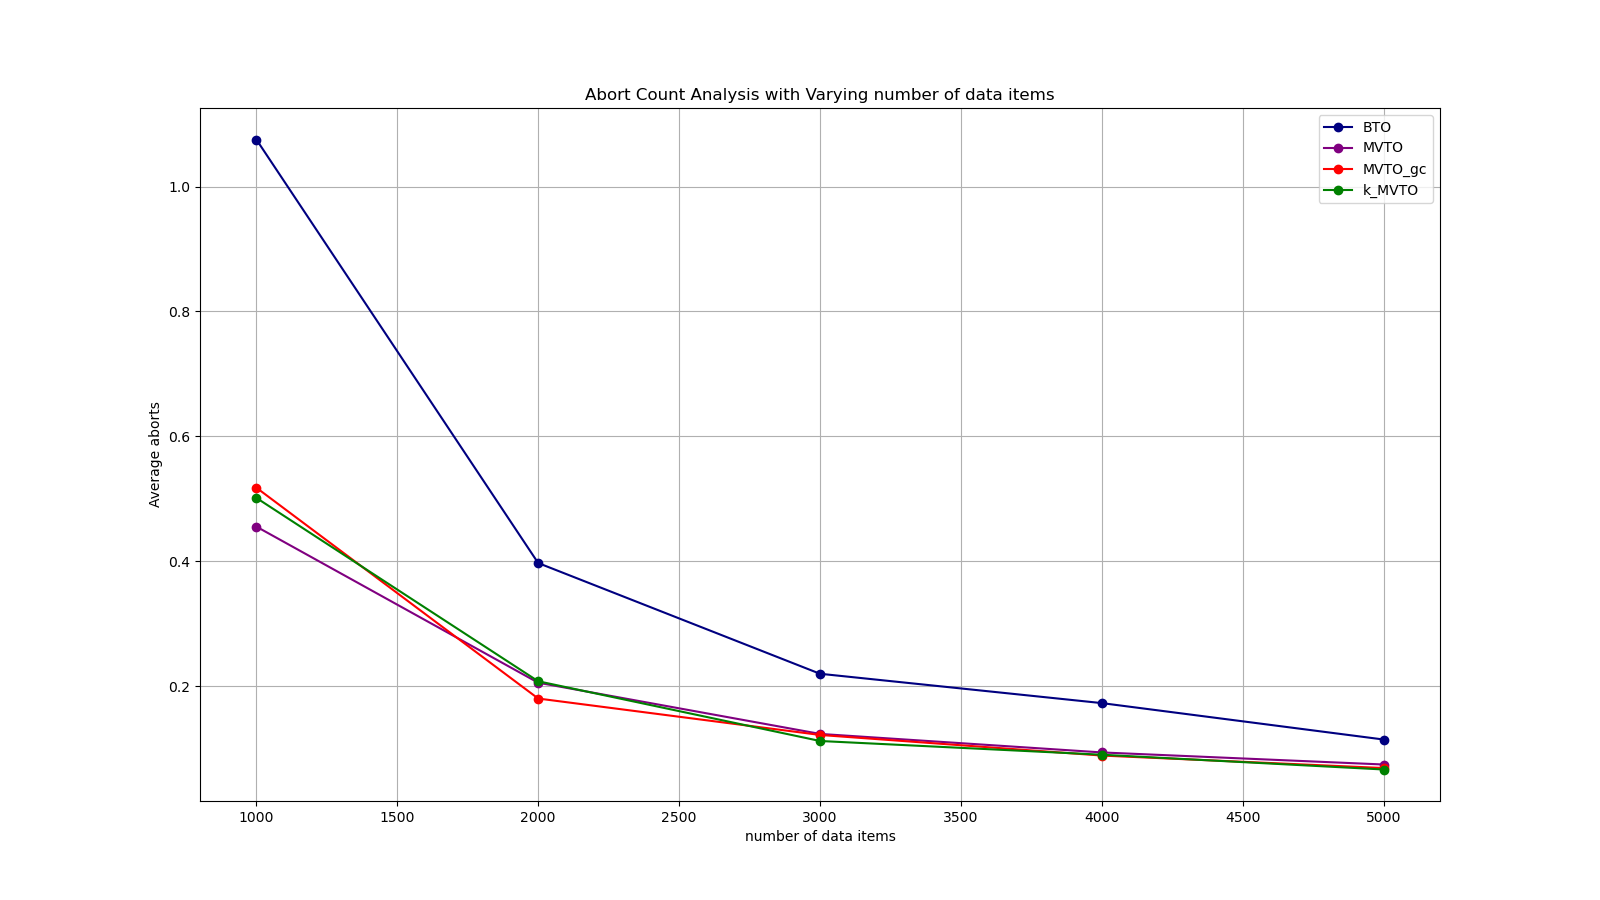
\includegraphics[width=0.9\linewidth]{img/E2_abortCount.png}
\end{figure}

\begin{figure}[h]
    \centering
    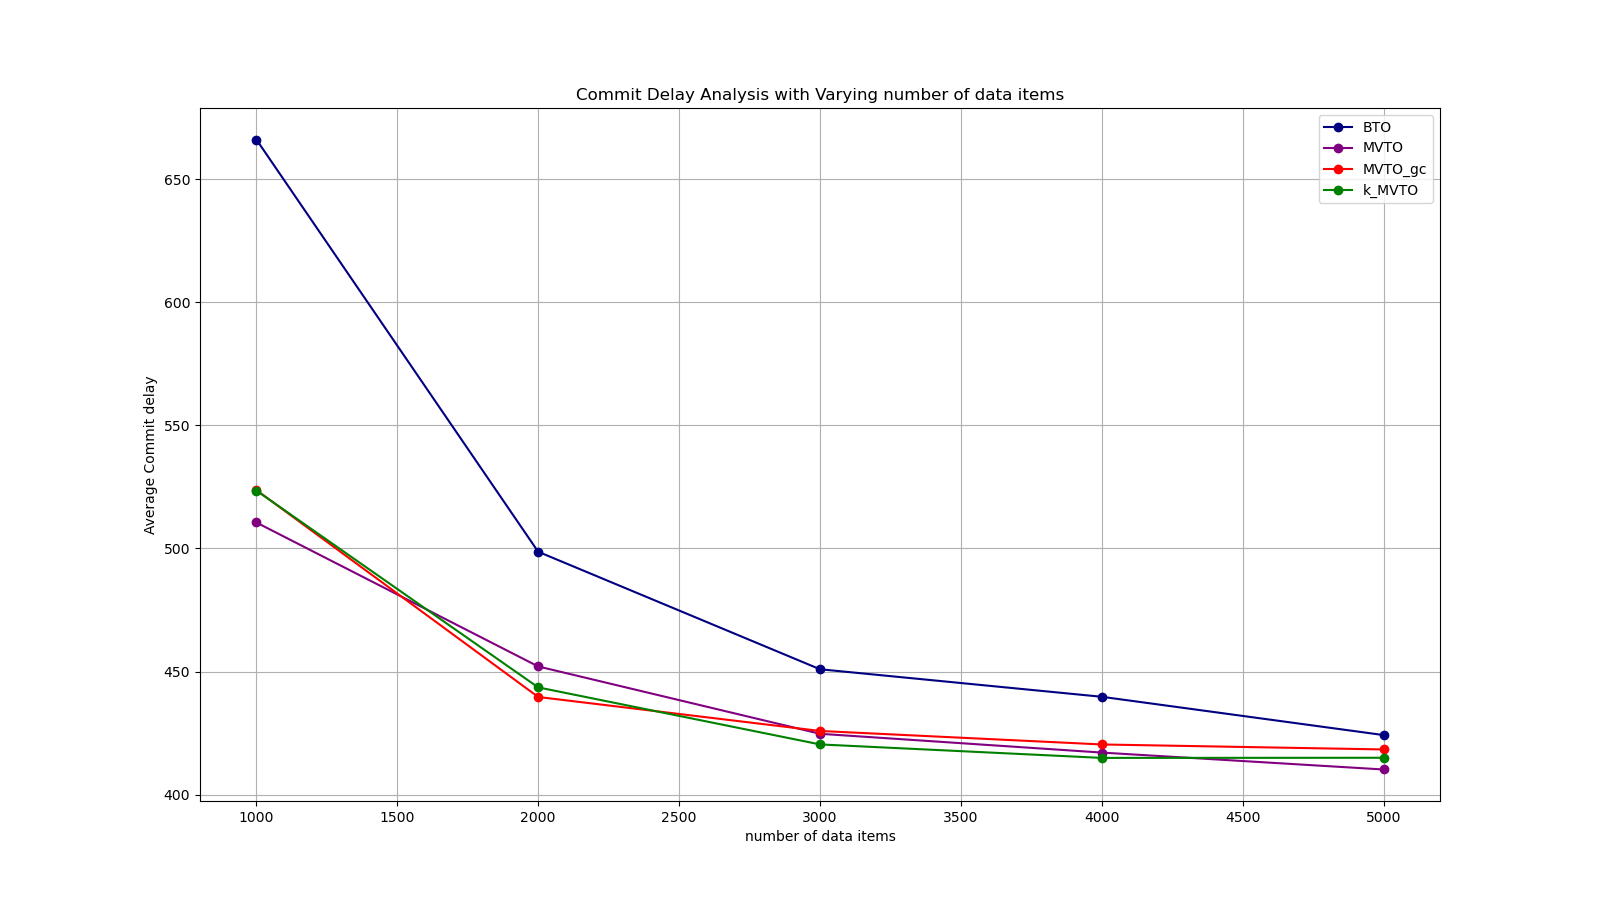
\includegraphics[width=0.9\linewidth]{img/E2_commitDelay.png}
\end{figure}
\paragraph{Explanation} 
By increasing the number of data items, we can see that the abort count and commit delays are rapidly decreasing. It is because when there are more data items, and when we are sampling the data items, we are decreasing the likelihood of same data item being picked by concurrent transactions, which reduce conflicts and thus reduce the abort counts and commit delays. We also see that the performance of BTO is still the worst, but the difference between the three MVTO variants is not that much.


\subsection{Experiment 3: Varying number of threads}
\begin{figure}[h]
    \centering
    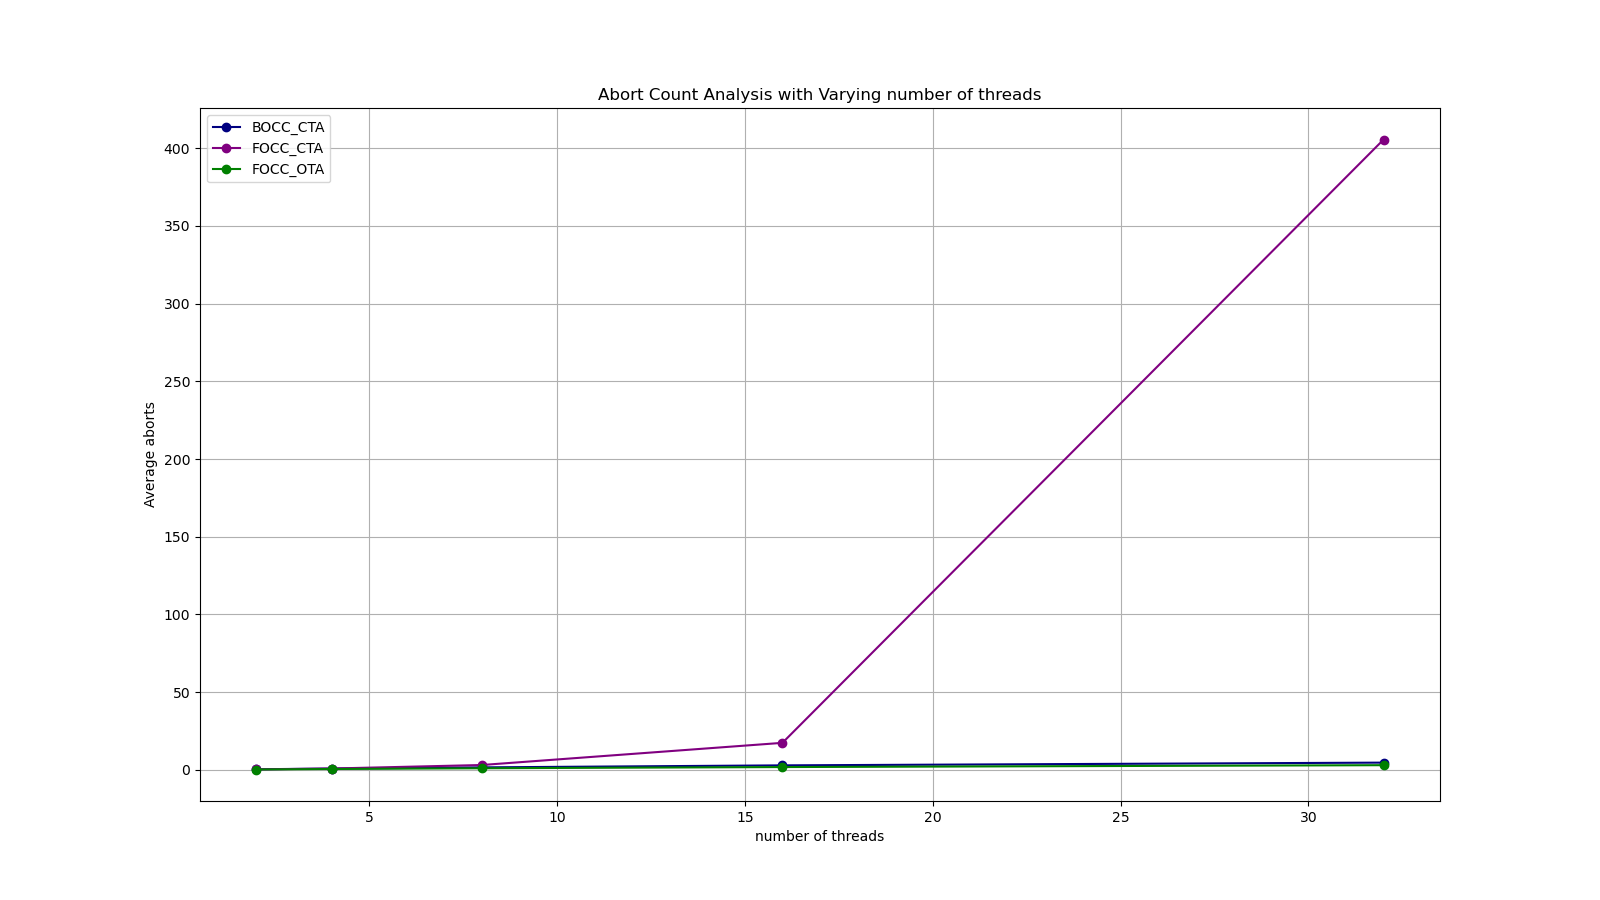
\includegraphics[width=0.9\linewidth]{img/E3_abortCount.png}
\end{figure}

\begin{figure}[h]
    \centering
    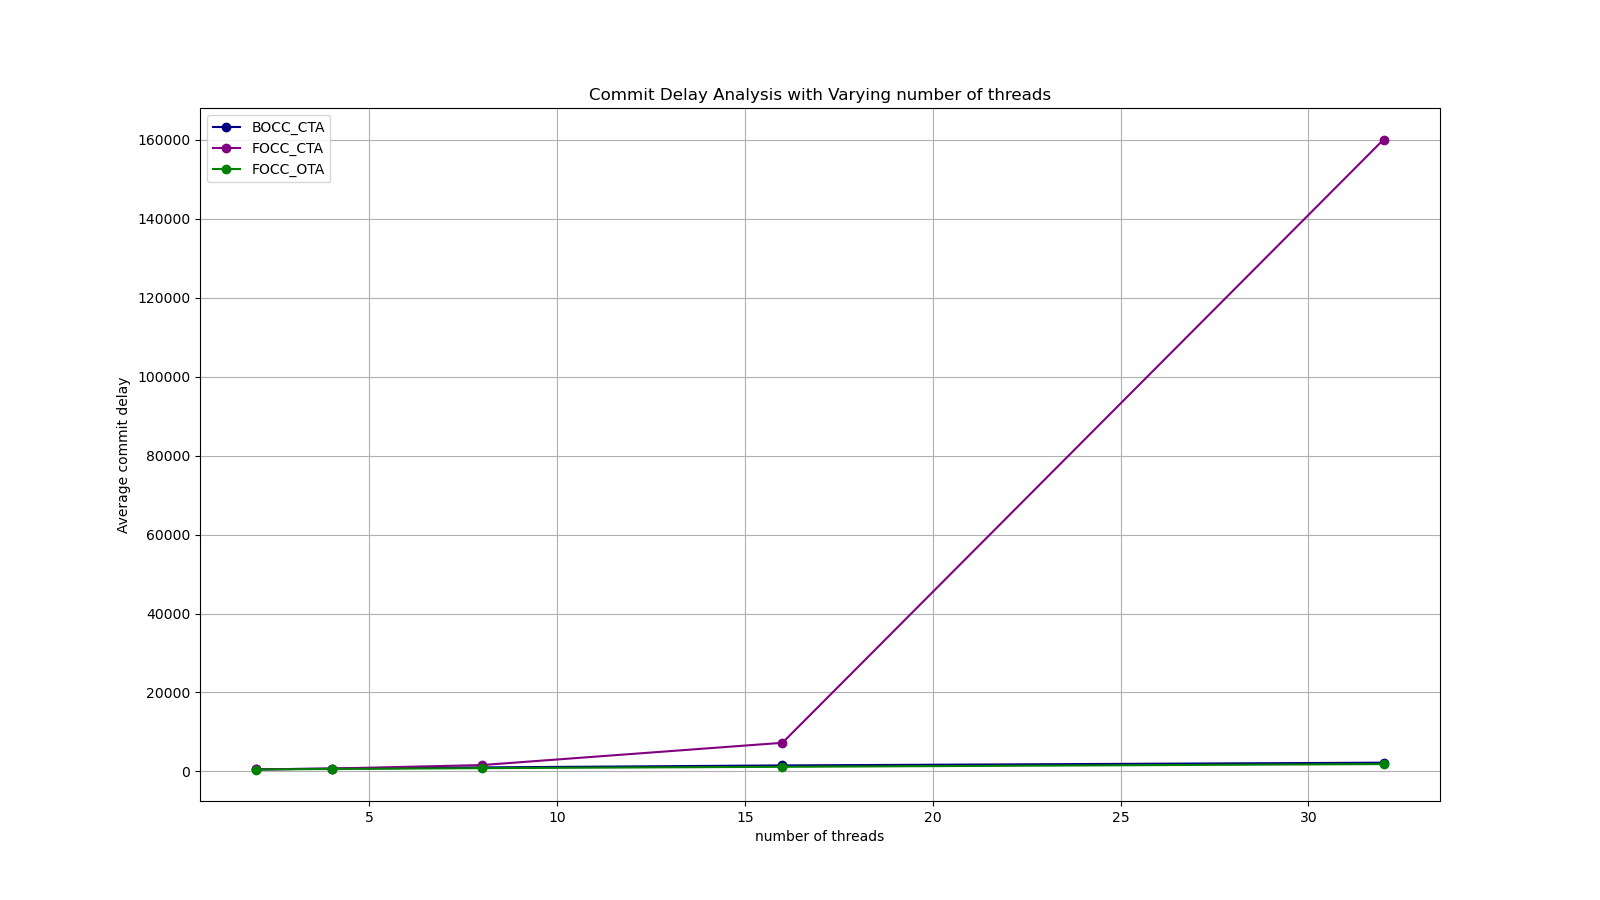
\includegraphics[width=0.9\linewidth]{img/E3_commitDelay.png}
\end{figure}

\paragraph{Explanation}
Usually we see that increasing threads improves performance because of a greater degree of concurrency. But in this case, by increasing the threads, we are increasing the number of concurrent transactions, not dividing work but we are creating more competition. When we have two threads, affectively only 2 transactions are running paralelly - chances they conflict are low, number of items to check are low and so on. Hence the result. If we were to measure the overall time taken for the programs to execute instead of abort count or commit delays, the result would've been different. Also, we can see that BTO doesnot scale well with the increasing number of threads, which is expected.


\subsection{Experiment 4: Varying value of k}
\begin{figure}[h]
    \centering
    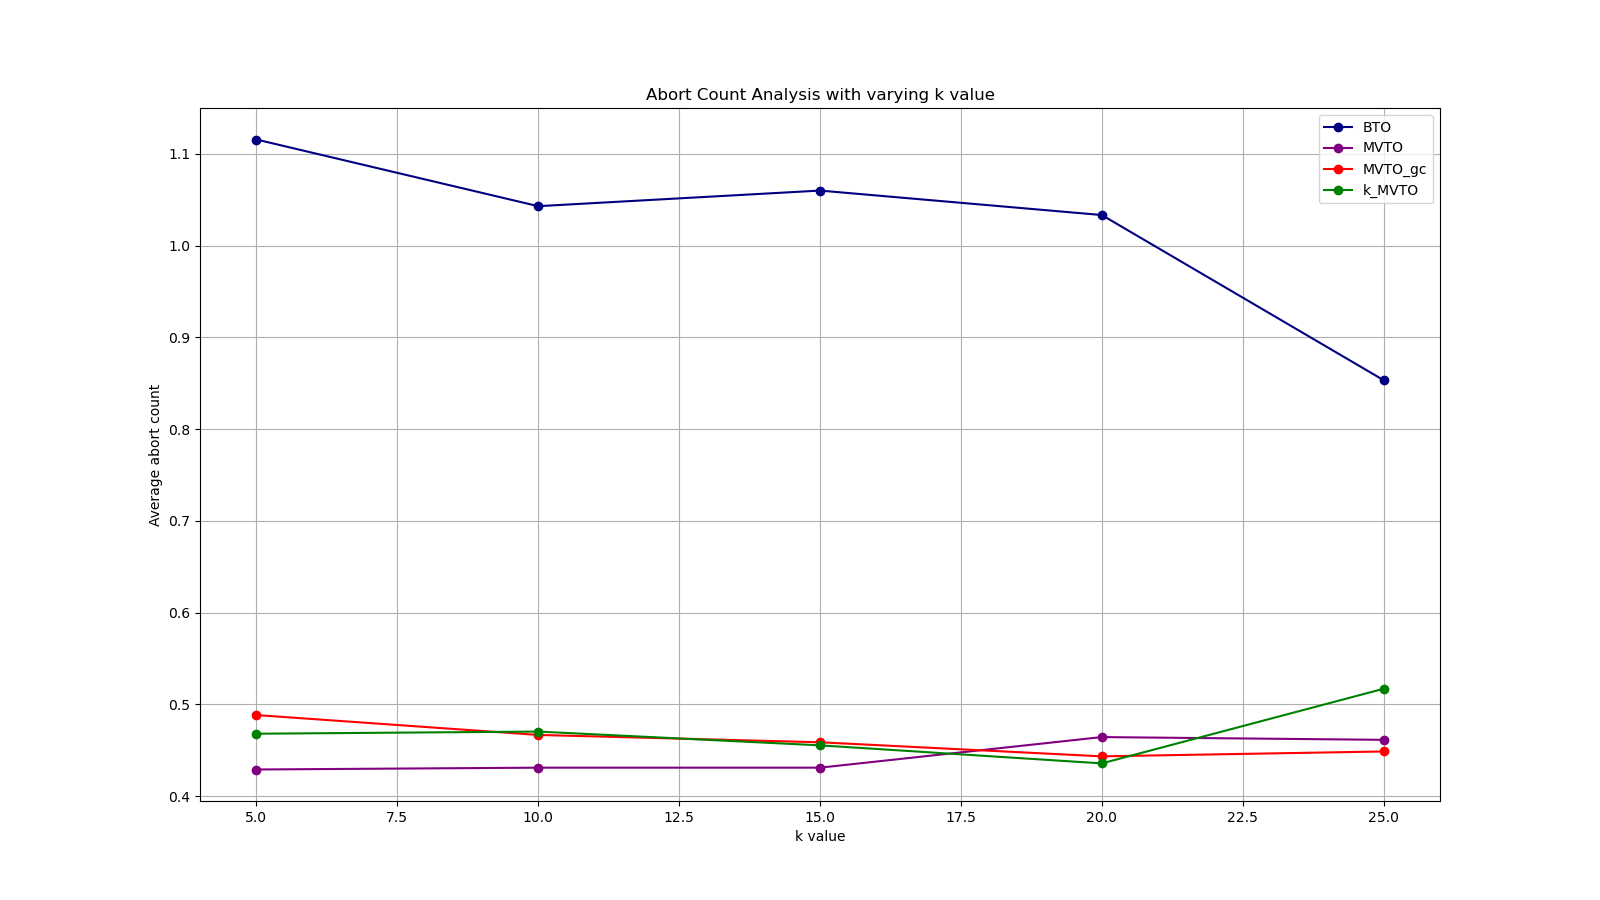
\includegraphics[width=0.9\linewidth]{img/E4_abortCount.png}
\end{figure}

\begin{figure}[h]
    \centering
    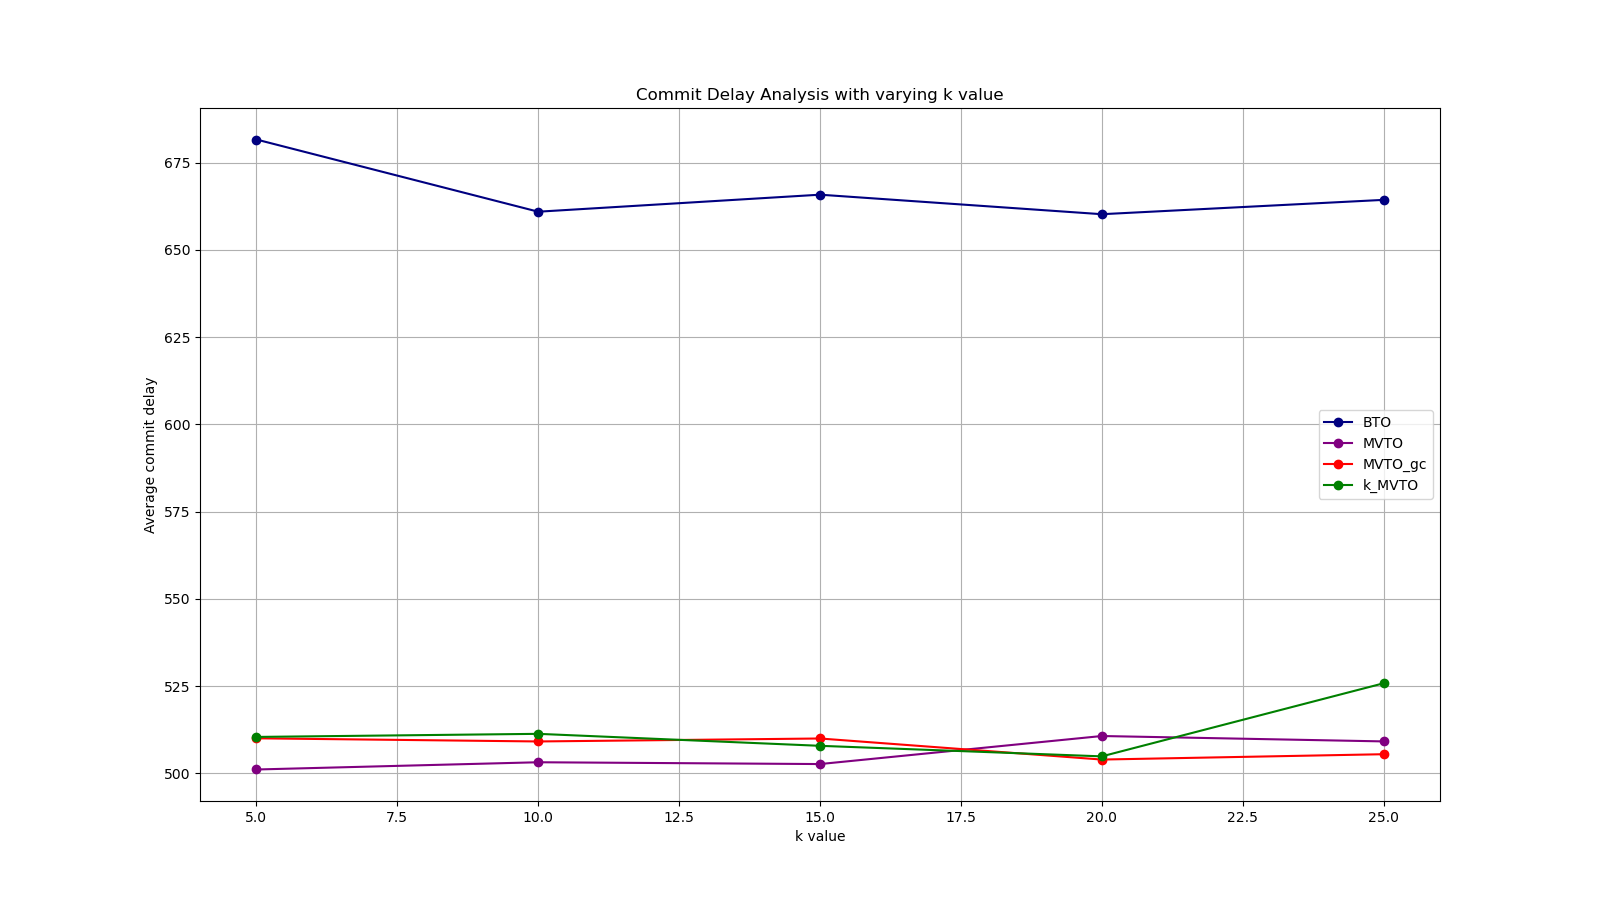
\includegraphics[width=0.9\linewidth]{img/E4_commitDelay.png}
\end{figure}

\paragraph{Explanation}
Specific to k-mvto, we see that it shows improvement as k increases, and we also see that it starts performing equal and even better than the mvto and mvto-gc at some values of k. And as usual, BTO is performing nowhere near, for any value of k of k-mvto.



\subsection{Experiment 5: Varying value of readRatio}
\begin{figure}[h]
    \centering
    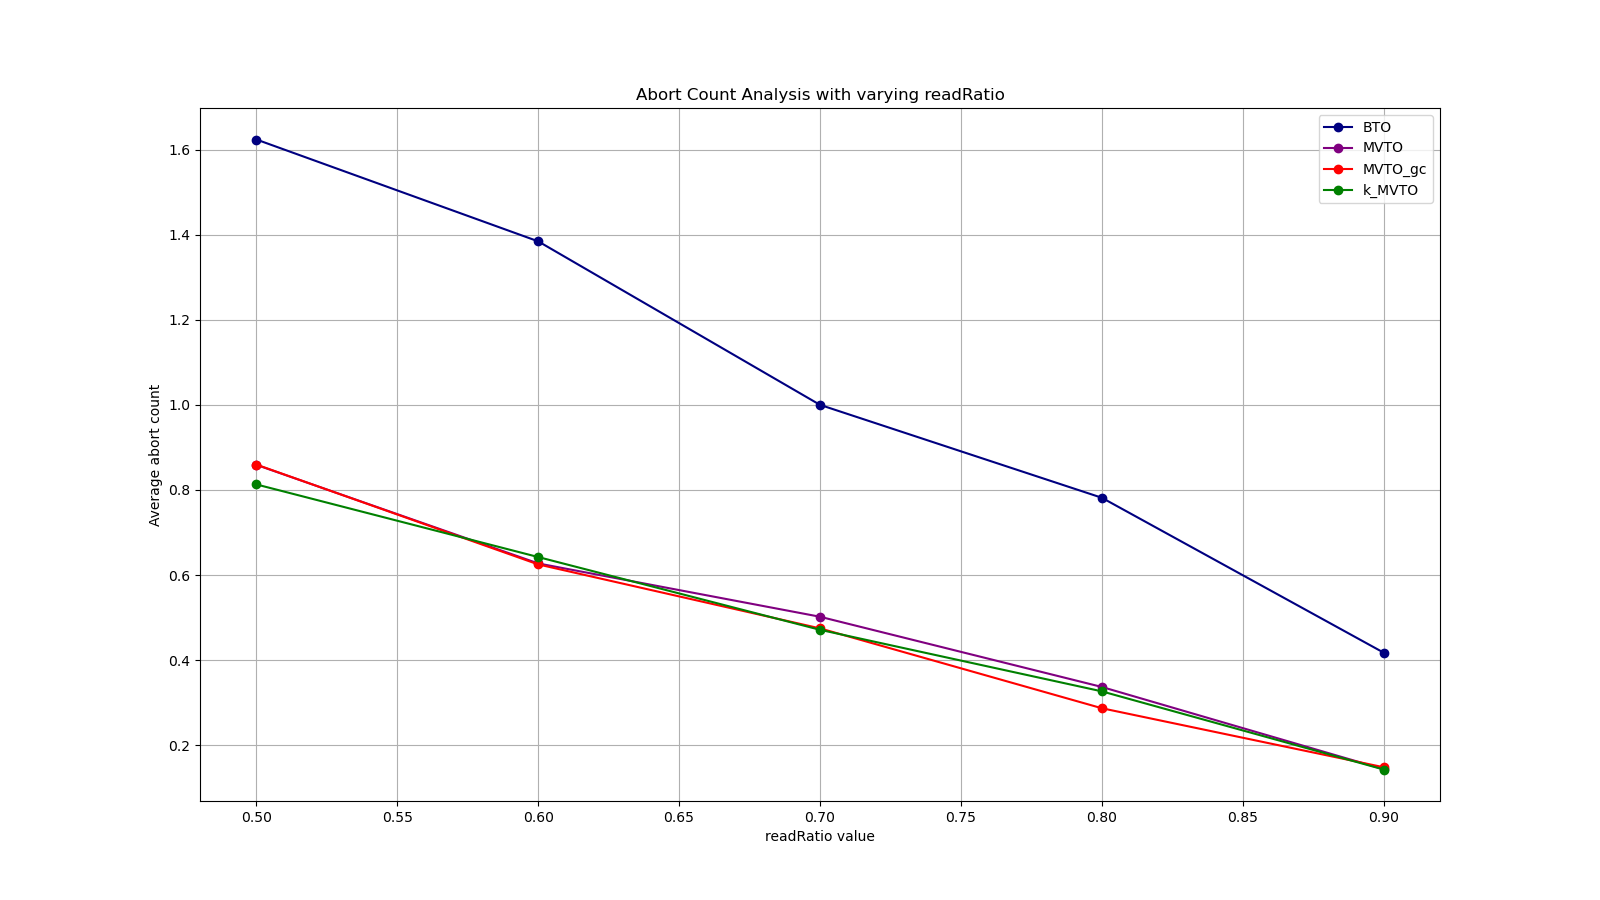
\includegraphics[width=0.9\linewidth]{img/E5_abortCount.png}
\end{figure}

\begin{figure}[h]
    \centering
    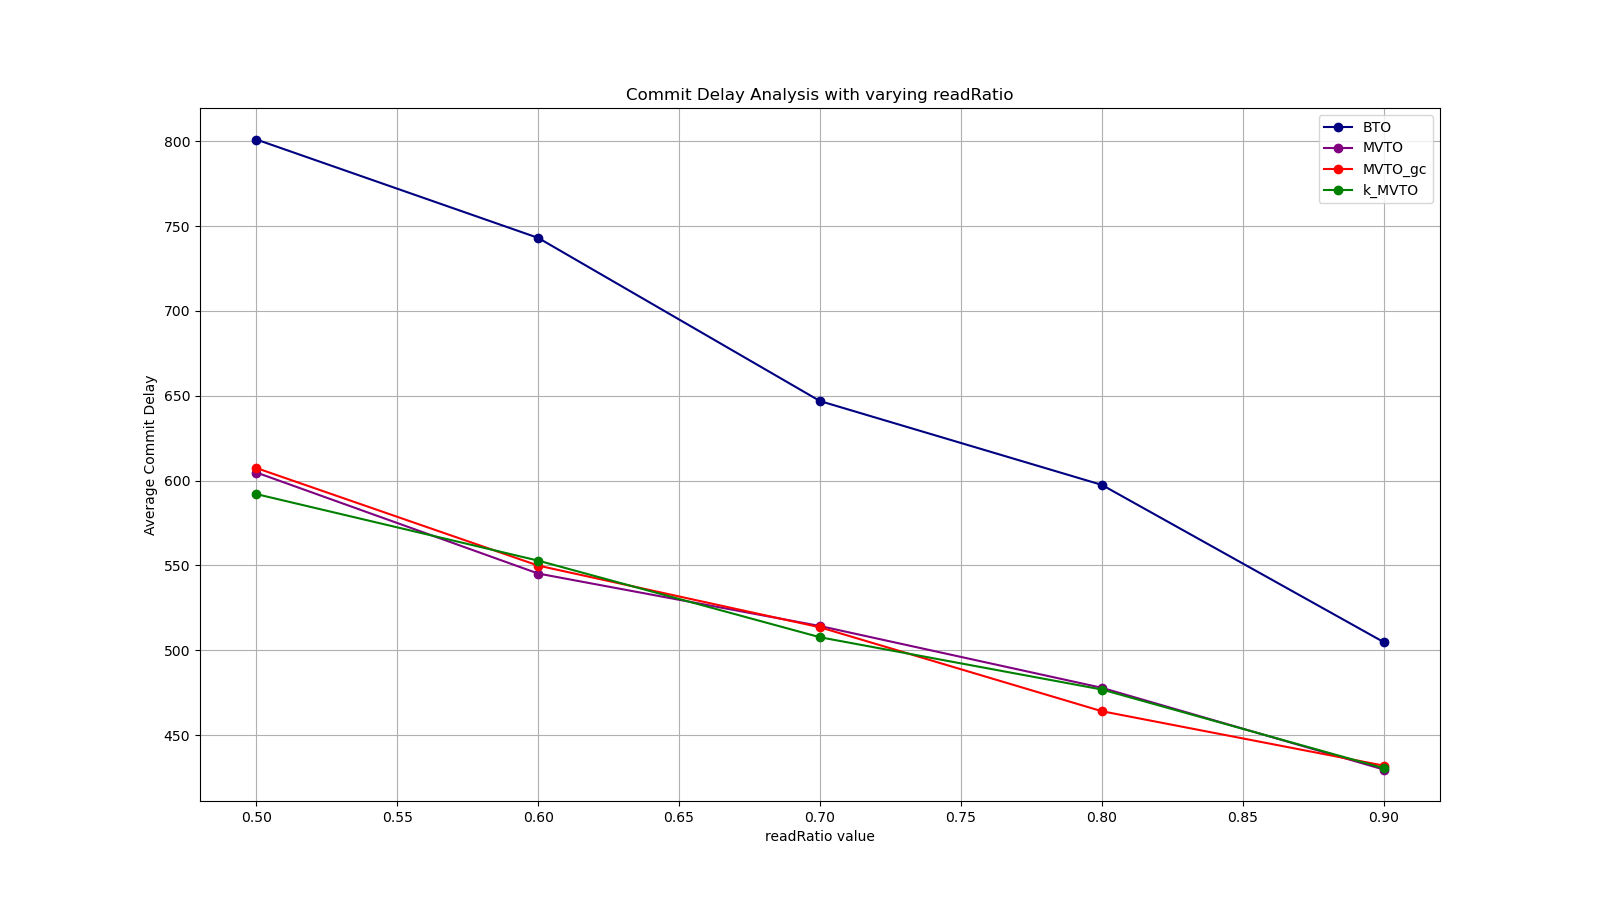
\includegraphics[width=0.9\linewidth]{img/E5_commitDelay.png}
\end{figure}
\paragraph{Explanation}
We see that with increased read ratio, the abort count and commit delay of all the algorithms are decreasing. This is expected because this significantly decreases the number of conflicts by avoiding read-write conflicts and write-write conflicts. We also see that mvto-gc is being able to take the best advantage of the increased read-ratio, which is expected because it avoids the iteration time for searching the right version, as well as avoids the aborts caused by not having the version needed.

\section{Future Work}
We can further improve the algorithm by using \textbf{binary search for finding the right version}, by keeping the sorted versions. This would exponentially decrease search time, and we can expect better results.


\end{document}
